\documentclass[a4paper]{article}


\usepackage[utf8]{inputenc}
\usepackage[T1]{fontenc}
\usepackage{textcomp}
\usepackage{mathtools,amssymb,amsthm}
\usepackage{lmodern}
\usepackage{geometry}
\geometry{hmargin=3cm,vmargin=3cm}
\usepackage{amsmath,amsfonts,amssymb}
\usepackage{tikz}
\usepackage{fancyhdr}
\usepackage{eso-pic}
\usepackage{xcolor}
\usepackage{listings}
\usepackage{booktabs}
\usepackage{setspace}
\definecolor{mGreen}{rgb}{0,0.6,0}
\definecolor{mGray}{rgb}{0.5,0.5,0.5}
\definecolor{mPurple}{rgb}{0.58,0,0.82}
\definecolor{backgroundColour}{rgb}{0.95,0.95,0.92}

\lstdefinestyle{customc}{
  belowcaptionskip=1\baselineskip,
  breaklines=true,
  frame=L,
  xleftmargin=\parindent,
  language=C,
  showstringspaces=false,
  basicstyle=\footnotesize\ttfamily,
  keywordstyle=\bfseries\color{green!40!black},
  commentstyle=\itshape\color{purple!40!black},
  identifierstyle=\color{blue},
  stringstyle=\color{orange},
}

\lstset{escapechar=@,style=customc}
\onehalfspacing
\begin{document}


\AddToShipoutPicture{%
  \AtPageLowerLeft{%
    \rotatebox{90}{\colorbox{gray!20}{%
      \begin{minipage}{\paperheight}\sffamily 
      \hspace*{\stretch{1}} \textbf{Rapport Projet S5: MANSUBA.}\hspace*{\stretch{1}}
      \end{minipage}%
    }}%
  }%
}


\title{  
\includegraphics[scale=0.09]{logo.png} \\ \underline{Rapport de projet S5:} \\ \textbf{MANSUBA} \\$\newline$ 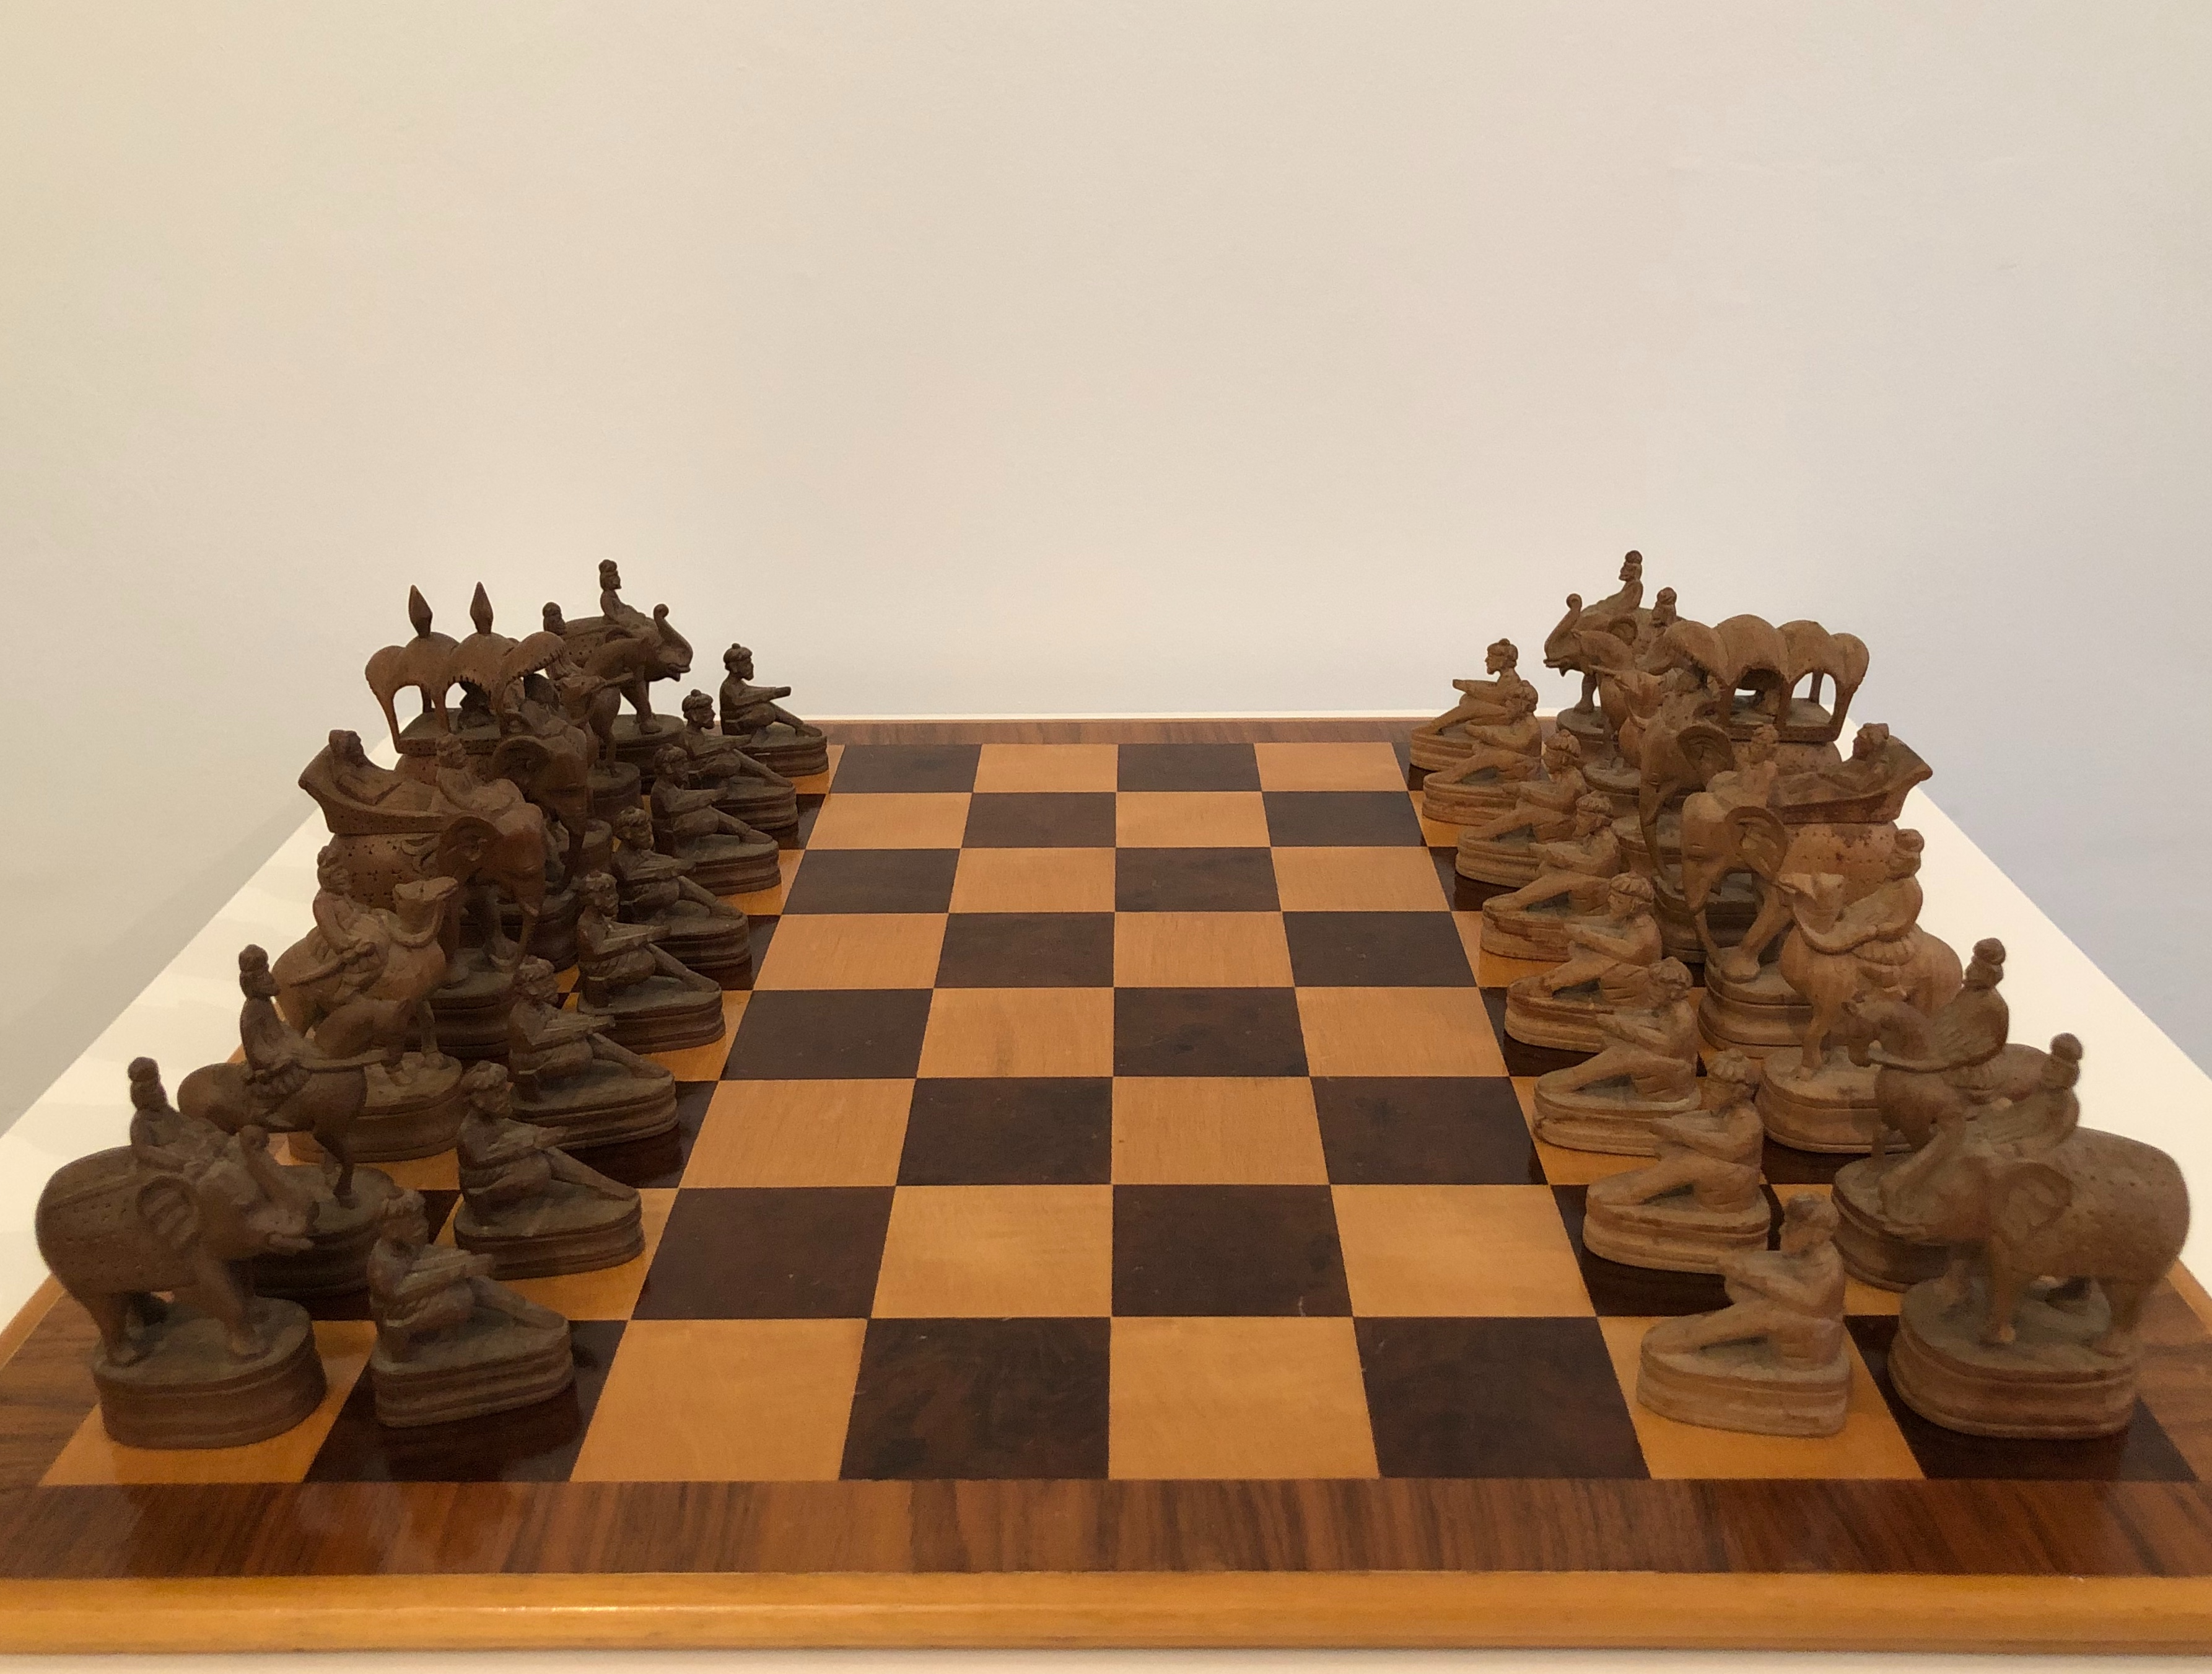
\includegraphics[scale=0.1]{Chaturanga_Chess_Set.jpg} }


\author{Réalisé par:\\MOHAMMED BOUHAJA ET AMIRA ELOUAZZANI \\\textbf{Encadré par: Julien Allali}}
\date{}
\maketitle





\newpage

\tableofcontents

\newpage



\section{INTRODUCTION}
\subsection{Problèmatique}
Mansuba est un jeu de plateau , ancêtre de Shtranj , qui a comme but mettre l’autre joueur en situation de mat . 
Le but de notre projet sera de jouer une partie aléatoire, puis rendre l'algorithme de plus en plus flexible
et l'orienter finalement vers la victory. 
\subsection{Hypothèse et démarches de validation}
Pour jouer une partie, il faut que le plateau de jeu soit définie au préalable. Le plateau de jeu \textit{board}  étant 
le binôme monde et relation. 
Le monde \textit{world} est l’set des cases accessibles par les pions et dont les mouvements seront permis . Chaque case a 
désormais des cases voisines \textit{Neighbors} dans des directions précisé par \lstinline|enum dir_t|.
\begin{lstlisting}
enum dir_t {
  NO_DIR  = 0,    // Default dir (i.e unset)
  EAST    = 1,
  NEAST   = 2,
  NORTH   = 3,
  NWEST   = 4,
  WEST    = -1,
  SWEST   = -2,
  SOUTH   = -3,
  SEAST   = -4,
  MAX_DIR = 9,    // Total number of different directions
};
\end{lstlisting}
La possibilité d’accès à ses voisins sera contrôlée par la relation de la partie et qui choisira parmis les voisins ceux qui sont
 accessibles par mouvement direct.  
 
 
 \begin{center}
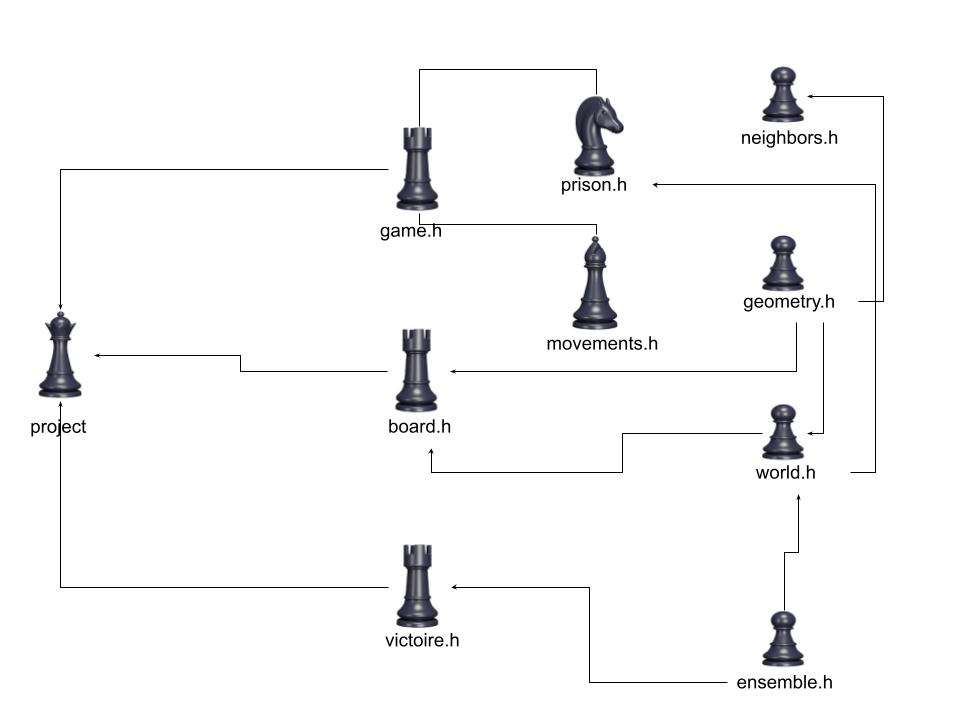
\includegraphics[scale=0.5]{Dessin sans titre.jpg} 

\end{center}

\section{Bases du jeu}




Le jeu s’effectue un monde de $\textcolor{purple}{\textsc{world\_size}} = \textcolor{purple}{\textsc{width}} \times 
 \textcolor{purple}{\textsc{height}}$  case , des pièces (\lstinline|enum sort_t|) pour les joueurs ayant la couleur 
 dans (\lstinline|enum color_t|) . Cette configuration est surtout gouvernée par \textcolor{green}{\textit{geometry.h}}. \\
\begin{lstlisting}
enum sort_t {
  NO_SORT  = 0,   // Default sort (i.e nothing)
  PAWN     = 1,
  TOUR     = 2,
  ELEPHANT = 3,
  MAX_SORT = 4,   // Total number of different sorts
};
enum color_t {
  NO_COLOR  = 0,  // Default color, used to initialize worlds
  BLACK     = 1,
  WHITE     = 2,
  MAX_COLOR = 3,  // Total number of different colors 
};
\end{lstlisting}

Pendant le développement du jeu on fera souvent appel à toute la configuration du jeu. On rassemble alors tous les paramètres du monde
 actuel pendant le jeu dans une structure \lstinline|struct game_t|.
\begin{lstlisting}
struct game_t {
    enum color_t current_player;
    unsigned int tour;
    struct world_t* w;
    struct jail_t* jail;
    unsigned int seed;
    unsigned int position;
    enum victory_t victory;
};
\end{lstlisting}
Pour jouer une partie aléatoire on aura besoin de configurer le plateau de jeu.
\subsection{Partie monde}
La structure world est un tableau de pair couleur et type de pions qui inaccessible que par des fonctions de 
\textcolor{green}{\textit{world.h}}. On commence d’abord par initier un monde sans aucun pion à l’aide de la structure 
\lstinline|struct world_t* world_init();|. Cette fonction attribue à chaque case du tableau monde le pair 
\textcolor{purple}{\textsc{(no\_color , no\_sort)}}. Les fonctions de world.h permettront l’écriture et la lecture de la couleur et
 du type d’une case donné et seront utilisé fréquemment pour accéder au monde.  
 
 \begin{center}
 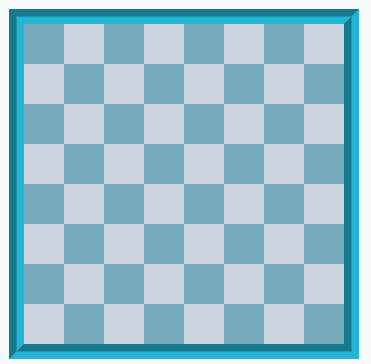
\includegraphics[scale=0.4]{boardvide.png}{\\$\hspace*{0.7cm}$Figure x: Un monde avec 64 cases indexées de 0 à 63.}
 \end{center}

\subsection{Partie relation}



La structure \lstinline|struct neighbors_t| prédéfinira les voisins de chaque indice donné . 
\begin{lstlisting}
struct neighbors_t {
  struct vector_t n[MAX_NEIGHBORS+1];
};
\end{lstlisting}

\begin{center}
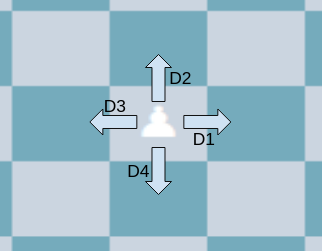
\includegraphics[scale=0.5]{movespawn2.png} {\\$\hspace*{0.7cm}$Figure x: }
\end{center}


Les voisins seront un tableau dont le contenu pour un indice donné est un tableau de vecteur introduit par la structure \lstinline|struct vector_t| défini par l’indice
 du voisin et sa direction de taille \textcolor{purple}{\textsc{max\_neighbors}} . De la même façon que world, les fonctions qui donne 
 accès au voisins sont \lstinline|struct neighbors_t get_neighbors(unsigned int idx)| qui cherche dans la structure des voisins 
 l’élement d’indice rentré en paramètre et \lstinline|unsigned int get_neighbor(unsigned int idx, enum dir_t d)|qui aide à obtenir 
 le voisin dans une direction donné par des opérations sur l’indice.\\ 

L’initialisation d’une relation modifie la liste des voisins pour qu’il puisse inclure que des voisins de certain directions donné. 
Avant d’initialiser une relation on pose dans la structure neighbors comme premier voisin pour chaque indice le pair 
\textcolor{purple}{\textsc{(uint\_max , no\_dir)}} et un (0,0) pour le reste. \textcolor{purple}{\textsc{uint\_max}} est définie 
dans \textcolor{green}{\textit{limits.h}}. La fonction add\_neighbor servira par suite à pousser \textcolor{purple}{\textsc{(uint\_max , no\_dir)}} 
et le remplacer par le pair indice du voisin et sa direction.
\subsection{set}
\begin{lstlisting}
struct set{
    unsigned int taille;
    unsigned int positions[WORLD_SIZE];
};
\end{lstlisting}
Cette structure \lstinline|struct set|  permettra de construire des tableaux d’une taille donnée et simplifier leurs 
manipulations : lecture et écriture , comme le jeu a plusieurs collections à fournir : l’set des positions des pions, la 
collection des mouvement possibles (qui sera le but de l’étape qui suit) ... . Elle contient comme attribut un entier qui donne la 
taille et un tableau d'indice qui sont le contenu de l'set.
On a défini en plus une fonction qui sera utile pour le reste, add\_position, qui augmente la taille et remplace la position d’indice 
rentré en paramètre par sa valeur. 
\begin{lstlisting}
void add_position(struct set* p ,unsigned int place ){
    p->positions[p->taille]=place ;
    p->taille+=1;
}
\end{lstlisting}
\section{Mobilités des pièces}
\subsection{Mobilité d'un pion \textit{PAWN}}
Pour stocker les mouvements on fera appel à la structure set . Les mouvement possibles dans la version de bases sont :  

    \textbf{\textcolor{magenta}{Déplacement simple}} : pour les relever il suffit d’utiliser la fonction get\_neighbors pour un indice donné . Ils seront stockés par la fonction \lstinline|void simple_moves( struct game_t game, struct set* sm );|
    
    
\begin{center}
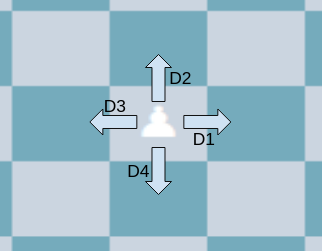
\includegraphics[scale=0.5]{movespawn2.png} {\\$\hspace*{0.7cm}$Figure x: Déplacement simple d'un pion.}
\end{center}

$\newline$

    \textbf{\textcolor{magenta}{Saut simple}} : si le voisin dans une direction j est occupé, équivalent d’avoir la fonction get\_neighbor dans la direction j qui a un SORT différent de NO\_SORT, et le voisin du voisin dans la meme direction est libre ,  on peut se déplacer vers le voisin du voisin , si le monde le permet. Ils seront stockés par la fonction \lstinline|void simple_jumps(struct game_t game , struct set* sj);|
    
    \begin{center}
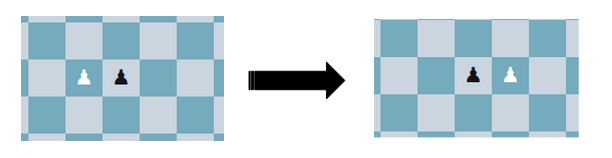
\includegraphics[scale=0.6]{sautf.png} {\\$\hspace*{0.7cm}$Figure x: Saut simple d'un pion.}
\end{center}

$\newline$

    \textbf{\textcolor{magenta}{Saut multiple}} : s’agit d’une suite de saut simple . Cette fonction avait besoin d’une condition d’arrêt pour éviter de boucler infiniment sur les sauts simples autre que les deux voisins soient occupés. Pour cela il nous fallait une fonction qui vérifie l’existence d’un élément dans un set donné \lstinline| int place_visited(struct set* ens, unsigned int place );|Elle renvoie un 0 si la place n’est pas encore mentionnée dans l’set qui sera notre condition pour arrêter la recherche. Ils seront stockés par la fonction \lstinline|void multiple_jumps(struct game_t game , struct set* mj )|.
    
\begin{center}
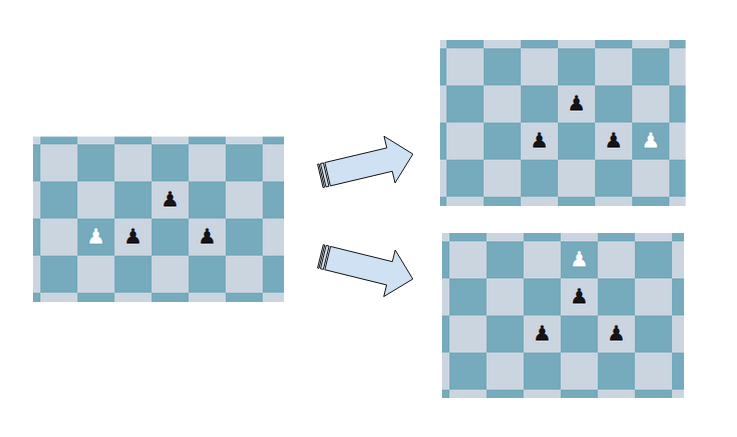
\includegraphics[scale=0.6]{sautmf.png} {\\$\hspace*{0.7cm}$Figure x: Saut multiple d'un pion.}
\end{center}

$\newline$

Ses fonctions prennent comme paramètre additionnel un set. Il servira comme espace de stockage pour chacune des fonctions au lieu de retourner l’set à la fin de chacune . En plus, la fonction \lstinline|void available_movements(struct game_t game, struct set* am) |fera appel à toutes les fonctions de mouvement citée au-dessus et l’set rentrer comme paramètre dans cette fonction sera le même rentrer dans tous les fonctions pour qu’on puisse stocker tous les mouvements dans un même set.  
\subsection{Mobilité des autre pièces \textit{TOWER} et \textit{ELEPHANT }}

$\newline$

\textbf{\textcolor{magenta}{Translation cardinale}} : La tour se déplace en ligne droite soit horizontalement soit verticalement de tout nombre de cases inoccupées, donc on réalise une boucle sur les quatres direction SOUTH, NORTH, EAST et WEST, et on ajoute les position libre dans l'ensemble $ct$ de la fonction  \lstinline|void cardinal_translations(struct game_t game, struct set* ct)| jusqu'à ce qu'elle atteigne le bord de l'échiquier ou qu'elle soit bloquée par une autre pièce. Elle ne peut passer au dessus d'une autre pièce.

\begin{center}
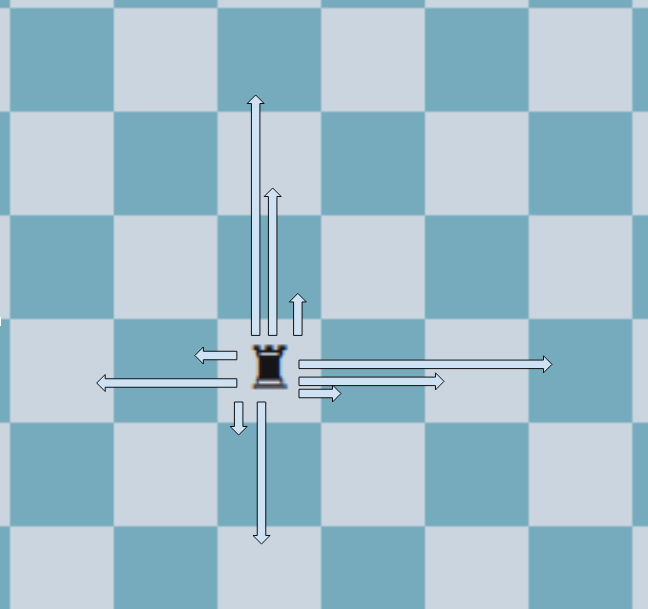
\includegraphics[scale=0.3]{tour2.png} {\\$\hspace*{0.5cm}$Figure x: Translation cardinal d'une tour.}
\end{center}

$\newline$

\textbf{\textcolor{magenta}{Saut semi diagonal}} : L'éléphant peut se déplacer sur les deux diagonale à partir de sa position initial, pour ce faire on boucle sur les directions $i+j$ $(où ~i \in \{NORTH, ~SOUTH\} ~et~ j \in \{ EAST, ~WEST \})$ et on ajoute les positions libres. finalement on stocke le résultat dans un ensemble $sdj$ à l'aide de la fonction \lstinline|void semi_diagonal_jumps(struct game_t game , struct set* sdj)|.

\begin{center}
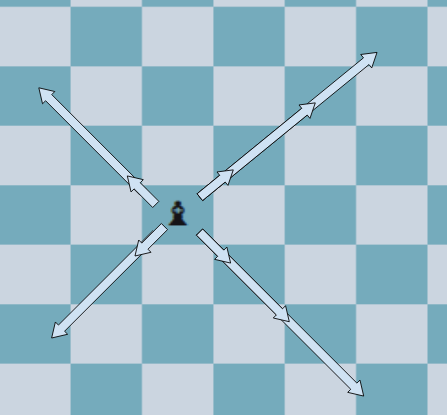
\includegraphics[scale=0.45]{ele2.png} {\\$\hspace*{0.4cm}$Figure x: Saut semi diagonal de l'éléphant.}
\end{center}


\subsection{Possibilité de capture et les tentatives d'évasion}
$\newline$

\textbf{\textcolor{magenta}{Capture simple}} :

$\newline$

\textbf{\textcolor{magenta}{Tentatives d'évasion}} :

\section{Boucle de jeu}
Le monde étant inacessible par d’autre document autre que \textcolor{green}{\textit{world.h}}. On a utilisé les fonctions
 \lstinline|void world_set(struct world_t* b, unsigned int idx, enum color_t c)| et \lstinline|void world_set_sort(struct world_t* b, unsigned int idx, enum sort_t c)|
 pour donner à un monde initialisé vide des positions pour chacun des pions. Le nombre des pions étant \textcolor{purple}{\textsc{height}}.  

Il existe deux types de victorys. La victory est dite simple si le joueur atteint une des positions de départ de l’autre joueur
 et complexe si le joueur les atteint tous. En tous cas, on aura besoin de garder la liste de positions de départ des deux joueurs 
 et leurs faire rentrer en paramètre pour pouvoir comparer avec les positions actuelles de l’adversaire. En plus, pour la comparaison on 
 pourra utiliser la fonction place\_visited. 

Le jeu s’arrête si on atteint une victory, le choix du type étant aléatoire pendant la partie, ou si on atteint \textcolor{purple}{\textsc{max\_turns}}. 

Avant d’obtenir la boucle de jeu finale il faudra définir des fonctions qui font des choix aléatoires sur tous les paramètres du jeu. 
Le choix du pion sera fait par \lstinline|void choose_random_piece_belonging_to(struct game_t* game) |qui retournera un indice. La fonction \lstinline| unsigned int choose_random_move_for_piece(struct game_t game)| va chercher entre les mouvements disponibles pour cet indice et va ensuite choisir un indice auquel le pion va bouger. La fonction \lstinline|void move_piece(struct game_t game, unsigned int dst)| agira sur le monde et échangera l’état de la case à l’indice initial avec celle de l’indice du mouvement. On choisira ainsi aléatoirement le premier joueur à commencer. 

Dans cette partie on cherche à rendre le jeu de plus en plus générique pour qu'il nous offre plus de possibilités. La version initaile (2) est un peu basique car il contient le même type de pièces avec les mêmes déplacements.
Alors dans la suite on va essayer en premier temps de définir plusieurs types de pièces(Tour, Éléphant) avec de nouveau mouvements possibles(translation cardinal et saut semi-diagonal), avant de passer , et finalement ajouter la possibilité de capturer les pièces du joueur adversaire pour que la partie soit plus intéréssante et amusante.


\section{Configuration de compilation et exécution}
\subsection{Makefile}


Les fichier .c décrivent dans ce rapport ont été construit et exécuté à l'aide d'un Makefile. Ce fichier de configuration automatise les tâches de compilation et d'exécution, facilitant ainsi la maintenance et l'extensibilité du logiciel. Les options de compilation et les dépendances ont été définies dans le Makefile, ainsi que les cibles pour construire et exécuter le programme. Nous avons utilisé GNU Make, un outil populaire pour créer des Makefiles, pour créer le Makefile de ce projet. En cours de développement, nous avons rencontré des problèmes avec les dépendances de bibliothèques, qui ont été résolus en ajoutant des options de compilation supplémentaires dans le Makefile. La méthodologie de compilation et d'exécution décrite ici a permis un développement efficace et une exécution stable de tous les fichiers.

\subsection{La manipulation des options de ligne de commande}


Pour manipuler la ligne de commande on a utiliser $getopt$, c'est un moyen efficace pour la gestion des optiosn et des arguments lors de la compilation du projet, donc l'utilisation de getopt nous a permis de rendre le terminal une interface utilisateur intuisive et personnalisable. Il utilise une bibliothèque standard $getopt$ de C. Se qui nous a permis de définir avant l'éxusion du projet le type de victoire souhaité par l'utilisateur, le nombre de tours et le nombre qui génére $rand()$. 

La bibliothèque getopt en C utilise la fonction getopt() pour analyser les options et les arguments passés à un programme lors de son exécution. Cette fonction prend en entrée les arguments standard argc et argv du programme, ainsi qu'une chaîne de caractères optstring qui définit les options valides pour le programme.

La fonction getopt() analyse ensuite les arguments dans argv en utilisant les options définies dans optstring. Pour chaque option valide détectée, getopt() retourne le caractère correspondant. Si une option nécessite un argument, celui-ci est stocké dans la variable globale optarg.

Les options peuvent être spécifiées de différentes manières. Les options courtes sont des caractères simples précédés d'un tiret (par exemple: -t pour le type de victoire et -m pour le nombre de tours). Les options longues sont des chaînes de caractères précédées de deux tirets (par exemple: --option).

Après avoir analysé tous les arguments, getopt() retourne -1 pour indiquer qu'il n'y a plus d'options valides. Les développeurs peuvent utiliser cette valeur pour itérer sur les options et les arguments restants.

Il est important de noter que getopt() modifie l'ordre des éléments dans argv pour les options traitées. Les arguments restants sont décalés vers le début de la liste argv.

\section{Références}



\end{document}